%!TeX program = xelatex
\documentclass[12pt,a4paper,UTF8]{ctexart}
\usepackage{SEUReport}

\begin{document}

\cover

\begin{abstract}
手写数字图像具有书写倾斜、类内差异大和类别边界非线性的特点，标准 K-means
的球形簇假设难以充分描述其流形结构。本文提出一种基于图像矩倾斜校正、局部尺度
谱图、模块度重启选择和邻域一致性细化的无监督聚类方法。首先利用二阶图像矩估计
水平剪切量并校正数字倾斜；随后构建自适应局部尺度的 k 近邻图，通过归一化图拉普拉斯
矩阵得到谱嵌入；在谱空间中执行自主实现的 K-means++，并以原始邻域图的模块度而非
欧氏惯性选择重启结果；最后通过邻域多数投票修正局部不一致样本。参数选择与模型训练
均不使用真实类别标签，标签仅用于实验结束后的客观评价。

在 scikit-learn Digits 数据集的 1797 幅图像上，本文方法取得 95.55\% 的聚类
准确率、92.35\% 的归一化互信息和 90.63\% 的调整兰德指数。10 个随机种子下的
平均准确率为 $95.59\%\pm0.02\%$。相较原始 K-means，准确率提高 16.36 个百分点；
消融实验表明各改进模块均产生正向贡献。

\textbf{关键词：}手写数字聚类；谱聚类；K-means++；局部尺度；模块度；DBSCAN
\end{abstract}

\newpage
\tableofcontents
\newpage

\section{选题背景}

\subsection{应用背景与重要性}

手写数字识别是模式识别的典型任务，可用于邮政编码读取、票据处理、表单录入和
档案数字化。实际数据往往缺少完整标签，而人工标注成本较高，因此无监督聚类可作为
数据预分类、异常检测和半自动标注的基础环节。

与监督分类不同，聚类算法只能依靠样本之间的结构关系发现类别。手写数字存在明显的
类内差异，例如同一数字的倾斜方向、笔画粗细和书写位置不同；同时也存在较强的类间
相似性，例如数字 1 与 7、3 与 8、4 与 9。该任务能够综合考察特征预处理、距离度量、
图模型、迭代优化和无监督评价等课程知识。

\subsection{问题定义}

给定图像集合 $\mathcal{X}=\{\boldsymbol{x}_i\}_{i=1}^{N}$，其中
$\boldsymbol{x}_i\in\mathbb{R}^{64}$ 为 $8\times8$ 灰度图像展开得到的向量，
目标是在训练时不访问真实标签的条件下，将全部样本划分为 $K=10$ 个簇。真实数字
标签仅用于实验结束后计算 ACC、NMI 和 ARI。

\subsection{选题依据}

课程评分同时强调完成度、创新度和原创度。本文选择手写数字图像聚类，原因如下：

\begin{enumerate}
    \item 数据规模适中，可在普通计算机上完整运行参数实验和消融实验；
    \item K-means、K-means++、DBSCAN、PCA、HOG 和本文核心谱图流程均可独立实现；
    \item 数据集带有评价标签，但训练阶段不依赖标签，便于客观比较不同聚类假设；
    \item 标准 K-means 存在明确局限，为图结构建模和无监督结果选择提供了改进空间。
\end{enumerate}

\section{相关算法}

\subsection{K-means 与 K-means++}

K-means 将每个样本分配到最近的聚类中心，并最小化簇内平方误差
\cite{macqueen1967}：
\begin{equation}
    J=\sum_{i=1}^{N}\left\|
    \boldsymbol{x}_i-\boldsymbol{\mu}_{z_i}
    \right\|_2^2,
\end{equation}
其中 $z_i$ 为样本 $i$ 的簇编号，$\boldsymbol{\mu}_{z_i}$ 为对应中心。算法交替执行
样本分配和中心更新，直到中心移动量低于阈值。K-means++ 按样本到已有中心的平方距离
进行概率采样，降低随机初始化产生较差局部解的概率\cite{arthur2007}。

K-means 计算简单，但隐含簇近似球形、尺度相近且可由欧氏中心表示的假设。手写数字
在像素空间中往往分布于弯曲的低维流形，因此该假设并不充分。

\subsection{DBSCAN}

DBSCAN 根据邻域半径 $\varepsilon$ 和最小邻域样本数
\texttt{min\_samples} 区分核心点、边界点与噪声点\cite{ester1996}。其优点是不需要
预先指定簇数，并能够发现非凸簇；缺点是对距离尺度和密度差异敏感。高维空间中的距离
集中现象会进一步增加 $\varepsilon$ 的选择难度。

\subsection{谱聚类}

谱聚类将样本表示为图节点，通过图拉普拉斯矩阵的特征向量获得低维嵌入，再对嵌入
进行聚类\cite{shi2000,ng2002}。与直接在像素空间执行 K-means 相比，谱方法能够利用
局部邻接关系描述非线性流形。不过，标准谱聚类通常采用固定邻域权重，对局部密度变化
较敏感，聚类离散化阶段也仍可能受到 K-means 局部解影响。

\section{本文方法}

\subsection{整体流程}

本文方法包含五个步骤：

\begin{enumerate}
    \item 使用二阶图像矩估计并校正每幅图像的水平倾斜；
    \item 构建带局部自适应尺度的 kNN 加权图；
    \item 对归一化图拉普拉斯矩阵进行特征分解，得到谱嵌入；
    \item 多次运行 K-means++，以图模块度选择最佳无监督划分；
    \item 在原始 kNN 邻域中执行有限步多数投票，修正局部不一致标签。
\end{enumerate}

\subsection{基于图像矩的倾斜校正}

设灰度图像为 $I(x,y)$，总灰度质量为 $m_{00}$，质心为 $(\bar{x},\bar{y})$。
计算中心矩
\begin{equation}
    \mu_{11}=\frac{1}{m_{00}}\sum_{x,y}
    (x-\bar{x})(y-\bar{y})I(x,y),
\end{equation}
\begin{equation}
    \mu_{02}=\frac{1}{m_{00}}\sum_{x,y}
    (y-\bar{y})^2 I(x,y).
\end{equation}
水平剪切系数定义为 $a=\mu_{11}/\max(\mu_{02},\epsilon)$，校正坐标为
\begin{equation}
    x'=x-a(y-\bar{y}).
\end{equation}
离散位置使用线性插值。该步骤降低同一数字因倾斜方向不同造成的像素距离。

\begin{figure}[H]
    \centering
    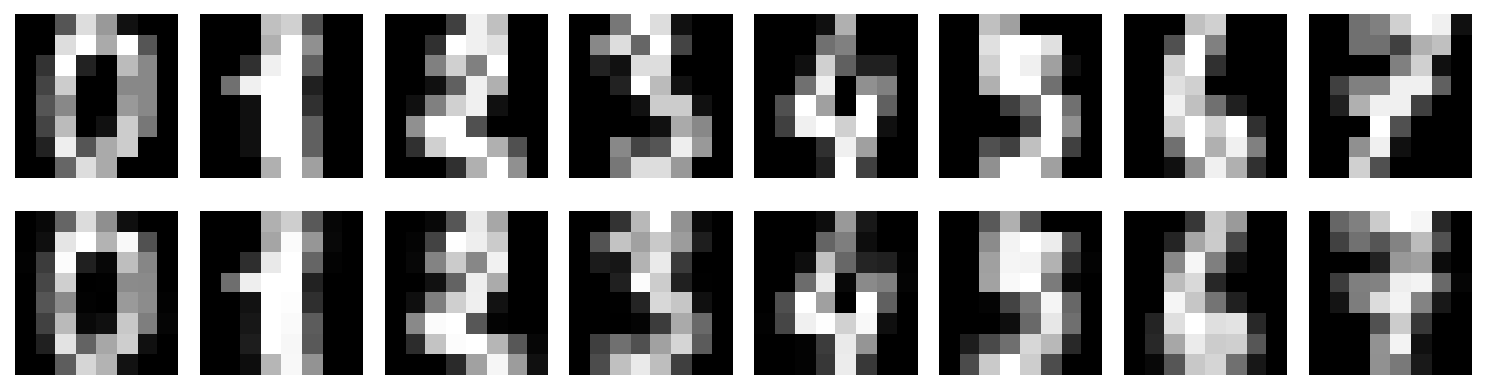
\includegraphics[width=0.92\textwidth]{figures/deskew_examples.pdf}
    \caption{原始图像与倾斜校正结果示例}
    \label{fig:deskew}
\end{figure}

\subsection{局部尺度 kNN 图}

对每个样本搜索 $k$ 个最近邻。固定高斯核带宽无法同时适应稠密区域和稀疏区域，
因此采用局部尺度思想\cite{zelnik2004}。令 $\sigma_i$ 为样本 $i$ 到其第 $l$ 个
近邻的距离，则有向边权为
\begin{equation}
    \tilde{w}_{ij}=
    \exp\left(-\frac{\|\boldsymbol{x}_i-\boldsymbol{x}_j\|_2^2}
    {\max(\sigma_i\sigma_j,\epsilon)}\right).
\end{equation}
本文使用并图进行对称化：
\begin{equation}
    w_{ij}=\max(\tilde{w}_{ij},\tilde{w}_{ji}).
\end{equation}
该设计既保留局部邻接，又避免互惠 kNN 图在小邻域下产生大量断开分量。

\subsection{归一化谱嵌入}

记邻接矩阵为 $W$，度矩阵为 $D$，其中
$D_{ii}=\sum_jw_{ij}$。构造对称归一化拉普拉斯矩阵
\begin{equation}
    L_{\mathrm{sym}}=I-D^{-1/2}WD^{-1/2}.
\end{equation}
取最小的 $K$ 个特征值对应的特征向量组成矩阵
$U\in\mathbb{R}^{N\times K}$，并对每一行进行 $\ell_2$ 归一化，得到谱嵌入
$Y$。该嵌入将图上连接紧密的样本映射到相近位置，使非凸结构更接近可由 K-means
划分的形态。

\subsection{基于模块度的重启选择}

普通 K-means++ 多次重启后通常选择谱空间惯性最小的结果。但实验发现，谱空间中的
最小欧氏惯性不一定对应原始图上的最佳分区。本文改为在每次重启后计算图模块度
\cite{newman2006}：
\begin{equation}
    Q=\sum_{c=1}^{K}\left[
    \frac{W(V_c,V_c)}{\sum_{i,j}w_{ij}}
    -\left(\frac{\operatorname{vol}(V_c)}
    {\sum_{i,j}w_{ij}}\right)^2
    \right],
\end{equation}
其中 $V_c$ 表示第 $c$ 个簇，$W(V_c,V_c)$ 为簇内边权之和，
$\operatorname{vol}(V_c)$ 为簇内节点度之和。最终选择 $Q$ 最大的重启结果。
该准则只依赖无标签邻域图，同时使离散化目标与谱建模目标保持一致。

\subsection{邻域一致性细化}

谱离散化后，少量边界样本可能与局部邻居标签不一致。对每个样本取最近的 $r$ 个
邻居，使用多数投票更新标签：
\begin{equation}
    z_i^{(t+1)}
    =\arg\max_c\sum_{j\in\mathcal{N}_r(i)}
    \mathbb{I}(z_j^{(t)}=c).
\end{equation}
本文仅执行有限步更新，避免过度平滑导致小簇被吞并。

\subsection{算法复杂度}

kNN 搜索在直接实现下约为 $O(N^2d)$；稀疏图特征分解主要与边数 $Nk$ 和目标
特征向量数 $K$ 有关；谱空间 K-means++ 每次迭代约为 $O(NK^2)$。Digits 数据集
规模较小，完整方法单次运行约 0.47 秒。对于更大数据集，可使用近似近邻搜索和
Nystr\"om 近似降低计算与存储成本。

\section{软件实现}

\subsection{开发环境}

实验环境为 Windows、Python 3.11、NumPy 2.4、SciPy 1.17、scikit-learn 1.9、
pandas 3.0 和 Matplotlib 3.10。项目使用 \texttt{uv} 管理依赖并生成锁文件。
报告使用 MiKTeX 25.12、XeLaTeX 和 BibTeX 编译。

\subsection{代码结构与原创性}

核心实现位于 \texttt{src/prml\_project/}：

\begin{itemize}
    \item \texttt{data.py}：加载 Digits 数据集；
    \item \texttt{features.py}：倾斜校正、HOG、PCA 和标准化；
    \item \texttt{clustering.py}：K-means、K-means++、DBSCAN 和本文谱方法；
    \item \texttt{metrics.py}：ACC、NMI、ARI、覆盖率等指标；
    \item \texttt{experiments.py}：基准、消融、敏感性、稳定性和图表生成。
\end{itemize}

K-means、K-means++、DBSCAN、PCA、HOG、局部尺度图、谱嵌入、模块度选择和邻域
细化均在项目中独立实现。scikit-learn 主要用于公开数据加载、标准指标，以及 GMM
和标准谱聚类外部基线。全部实验由配置文件控制，固定随机种子并输出 CSV。

\section{实验设计}

\subsection{数据集}

Digits 数据集包含 1797 幅 $8\times8$ 灰度手写数字图像，共 10 类，每个像素
取值范围为 0 至 16。程序加载后将其归一化到 $[0,1]$。数据集由 scikit-learn
内置提供，不需要额外下载，也不随最终代码提交。

\subsection{评价指标}

由于聚类编号与真实类别编号不存在固定对应关系，ACC 使用匈牙利算法寻找最佳一一
映射\cite{kuhn1955}。同时报告 NMI 和 ARI\cite{hubert1985}。对于 DBSCAN，还报告：

\begin{itemize}
    \item 全样本 ACC：噪声点计为错误；
    \item 条件 ACC：仅在非噪声样本上计算；
    \item 覆盖率：非噪声样本占全部样本的比例。
\end{itemize}

这种评价方式避免通过丢弃困难样本虚增 DBSCAN 准确率。

\subsection{参数与对比方法}

本文方法设簇数 $K=10$，候选近邻数
$k\in\{5,7,10,15,20,25,30\}$，局部尺度位置
$l\in\{1,2,3,5,7\}$。每组参数执行 100 次 K-means++ 重启，并按模块度选择结果。
参数 $(k,l)=(7,2)$ 在候选集合中取得最高模块度，因此无需真实标签完成选择。
邻域细化使用 5 个近邻并迭代 3 步。

对比方法包括原始像素 K-means、PCA K-means++、HOG K-means++、DBSCAN、
高斯混合模型和标准 kNN 谱聚类。DBSCAN 取
$\varepsilon=1.05$、\texttt{min\_samples}=3。

\section{实验结果与分析}

\subsection{总体结果}

\begin{table}[H]
    \centering
    \caption{不同聚类方法的全量实验结果}
    \label{tab:benchmark}
    \resizebox{\textwidth}{!}{
    \begin{tabular}{lrrrrrr}
        \toprule
        方法 & ACC & NMI & ARI & 轮廓系数 & 覆盖率 & 时间/s \\
        \midrule
        原始像素 K-means & 0.7919 & 0.7409 & 0.6658 & 0.1824 & 1.0000 & 1.093 \\
        PCA + K-means++ & 0.7930 & 0.7413 & 0.6671 & 0.2127 & 1.0000 & 0.577 \\
        HOG + K-means++ & 0.8013 & 0.6868 & 0.6324 & 0.0793 & 1.0000 & 1.016 \\
        DBSCAN + PCA & 0.7045 & 0.7787 & 0.6446 & 0.1110 & 0.8603 & 0.028 \\
        高斯混合模型 & 0.8353 & 0.8129 & 0.7279 & 0.2032 & 1.0000 & 2.483 \\
        标准谱聚类 & 0.8742 & 0.8466 & 0.7913 & 0.1764 & 1.0000 & 0.621 \\
        \textbf{本文方法} & \textbf{0.9555} & \textbf{0.9235} &
        \textbf{0.9063} & 0.1661 & 1.0000 & 0.466 \\
        \bottomrule
    \end{tabular}}
\end{table}

\begin{figure}[H]
    \centering
    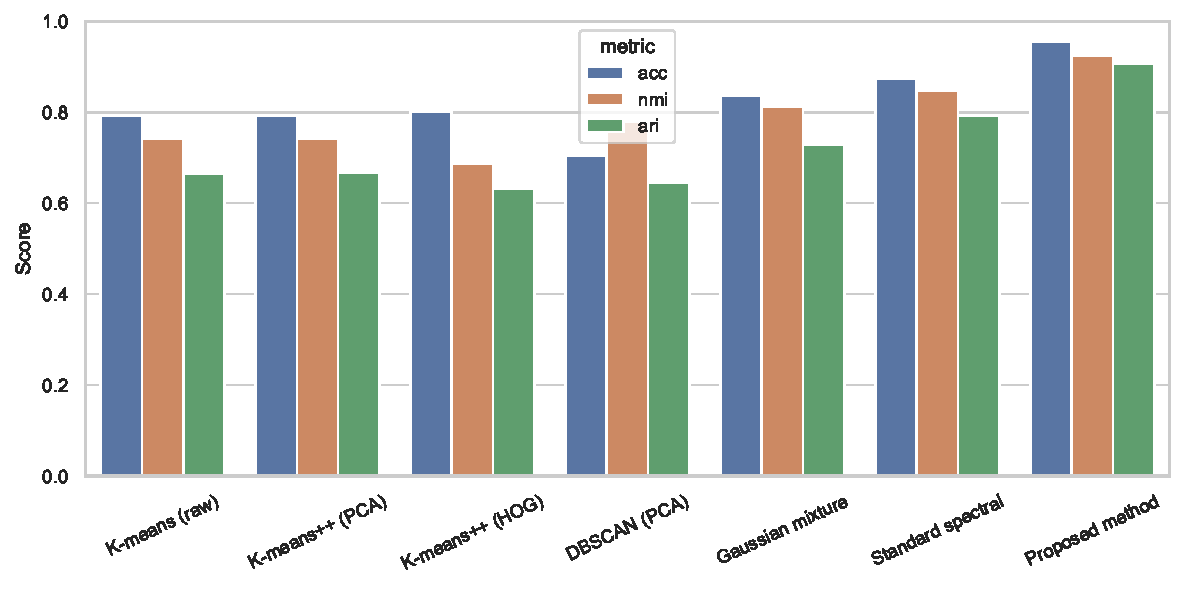
\includegraphics[width=0.92\textwidth]{figures/benchmark_metrics.pdf}
    \caption{不同方法的 ACC、NMI 和 ARI 对比}
    \label{fig:benchmark}
\end{figure}

本文方法的 ACC 比原始 K-means 提高 16.36 个百分点，比标准谱聚类提高
8.12 个百分点。这说明主要收益并非单纯来自谱分解，而是来自倾斜校正、局部尺度图、
模块度选择和邻域细化的共同作用。

轮廓系数最高的方法并非本文方法，这并不矛盾。轮廓系数基于当前特征空间中的欧氏
距离，而本文方法优化的是邻域图上的流形结构；手写数字类别不一定对应欧氏空间中的
球形高间隔簇。该现象也说明不能仅依赖单一内部指标评价聚类。

\subsection{DBSCAN 分析}

DBSCAN 的非噪声条件 ACC 为 0.8189，但覆盖率为 0.8603，全样本 ACC 下降到
0.7045，并产生 20 个簇而非 10 个簇。其 k-distance 曲线如
\autoref{fig:kdistance} 所示。结果表明 DBSCAN 能识别部分高密度核心样本，但不同
数字及不同书写风格的局部密度不一致，单一 $\varepsilon$ 容易同时产生簇碎裂和
噪声点。

\begin{figure}[H]
    \centering
    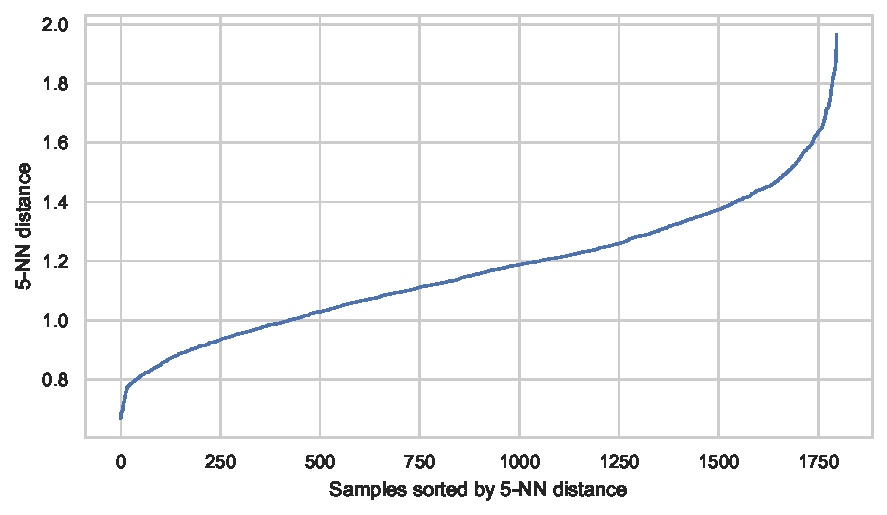
\includegraphics[width=0.68\textwidth]{figures/k_distance_curve.pdf}
    \caption{PCA 特征上的 5-NN 距离曲线}
    \label{fig:kdistance}
\end{figure}

\subsection{消融实验}

\begin{table}[H]
    \centering
    \caption{本文方法的逐模块消融结果}
    \label{tab:ablation}
    \begin{tabular}{lrrr}
        \toprule
        配置 & ACC & NMI & ARI \\
        \midrule
        A0：原始像素 K-means++ & 0.7919 & 0.7409 & 0.6658 \\
        A1：A0 + 倾斜校正 & 0.8002 & 0.7585 & 0.6811 \\
        A2：原图 + 局部尺度谱图 & 0.9087 & 0.8459 & 0.8066 \\
        A3：A2 + 倾斜校正 & 0.9149 & 0.8540 & 0.8199 \\
        A4：A3 + 邻域一致性细化 & \textbf{0.9555} & \textbf{0.9235} &
        \textbf{0.9063} \\
        \bottomrule
    \end{tabular}
\end{table}

\begin{figure}[H]
    \centering
    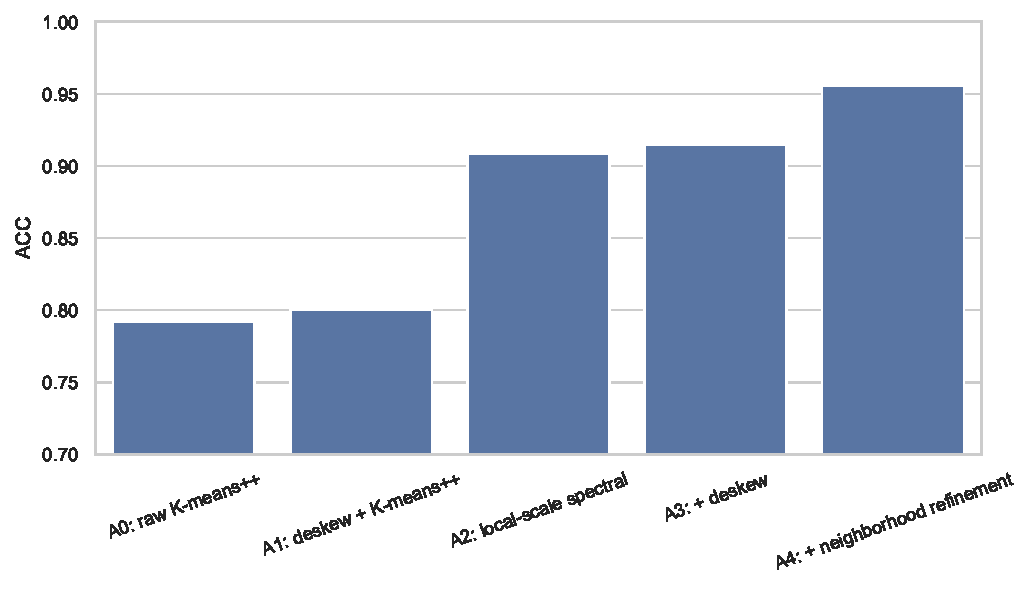
\includegraphics[width=0.86\textwidth]{figures/ablation_acc.pdf}
    \caption{逐模块消融实验的 ACC}
    \label{fig:ablation}
\end{figure}

局部尺度谱图贡献最大，使 ACC 从 0.7919 提高至 0.9087，说明数字图像的局部
流形关系比全局欧氏中心更适合该任务。倾斜校正在 K-means 和谱方法上均产生稳定增益。
邻域细化进一步提高 4.06 个百分点，表明谱离散化后的主要错误集中于局部边界样本。

\subsection{参数敏感性与无标签选择}

\begin{figure}[H]
    \centering
    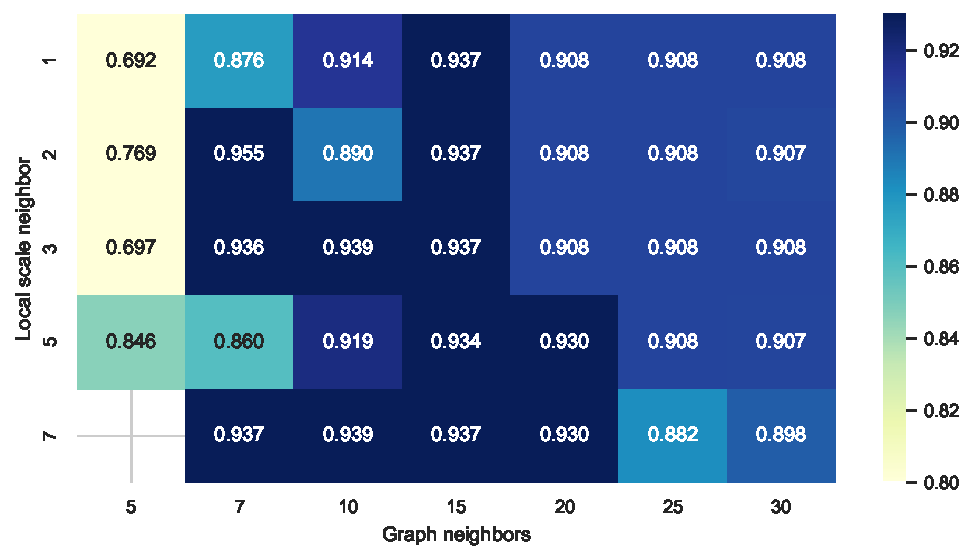
\includegraphics[width=0.78\textwidth]{figures/sensitivity_heatmap.pdf}
    \caption{近邻数与局部尺度位置的 ACC 敏感性}
    \label{fig:sensitivity}
\end{figure}

\begin{table}[H]
    \centering
    \caption{模块度较高的参数配置}
    \begin{tabular}{rrrrr}
        \toprule
        $k$ & $l$ & 模块度 $Q$ & ACC & NMI \\
        \midrule
        7 & 2 & \textbf{0.8924} & \textbf{0.9555} & \textbf{0.9235} \\
        7 & 7 & 0.8911 & 0.9366 & 0.8989 \\
        7 & 3 & 0.8893 & 0.9360 & 0.8971 \\
        10 & 3 & 0.8873 & 0.9393 & 0.9055 \\
        10 & 7 & 0.8870 & 0.9393 & 0.9055 \\
        \bottomrule
    \end{tabular}
\end{table}

候选配置中，最高模块度对应的 $(k,l)=(7,2)$ 同时取得最高外部评价结果，说明模块度
能够在不访问真实标签的条件下提供有效选择依据。过小的邻域可能导致图连接不足，
过大的邻域则会引入跨类别边，使局部流形结构被平滑。

\subsection{随机稳定性}

在随机种子 0 至 9 上重复完整实验，ACC、NMI、ARI 的均值和总体标准差分别为
\begin{equation}
    \mathrm{ACC}=0.95593\pm0.00022,
\end{equation}
\begin{equation}
    \mathrm{NMI}=0.92471\pm0.00060,\qquad
    \mathrm{ARI}=0.90735\pm0.00049.
\end{equation}
ACC 最小值为 0.95548，最大值为 0.95604。较小方差说明模块度重启选择显著降低了
K-means++ 初始化造成的不稳定性。

\subsection{混淆矩阵与误差分析}

\begin{figure}[H]
    \centering
    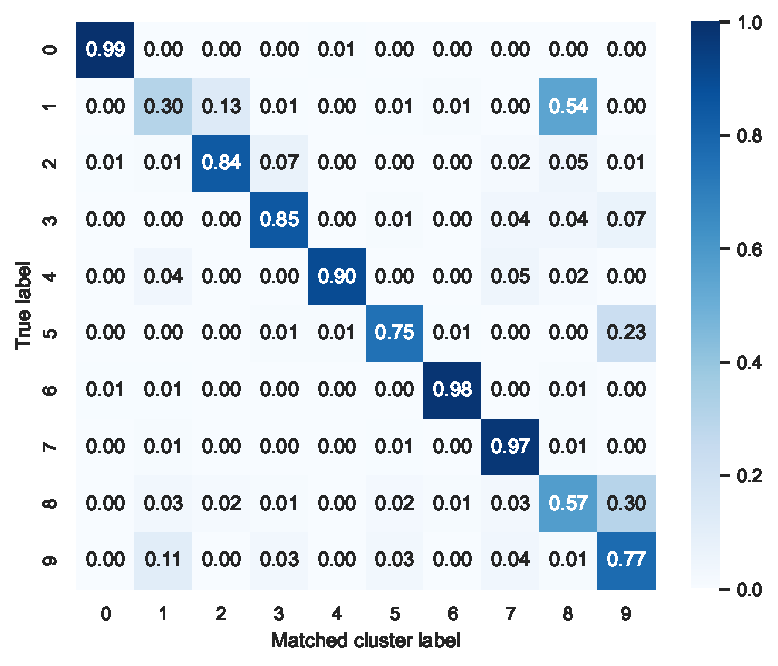
\includegraphics[width=0.48\textwidth]{figures/confusion_baseline.pdf}
    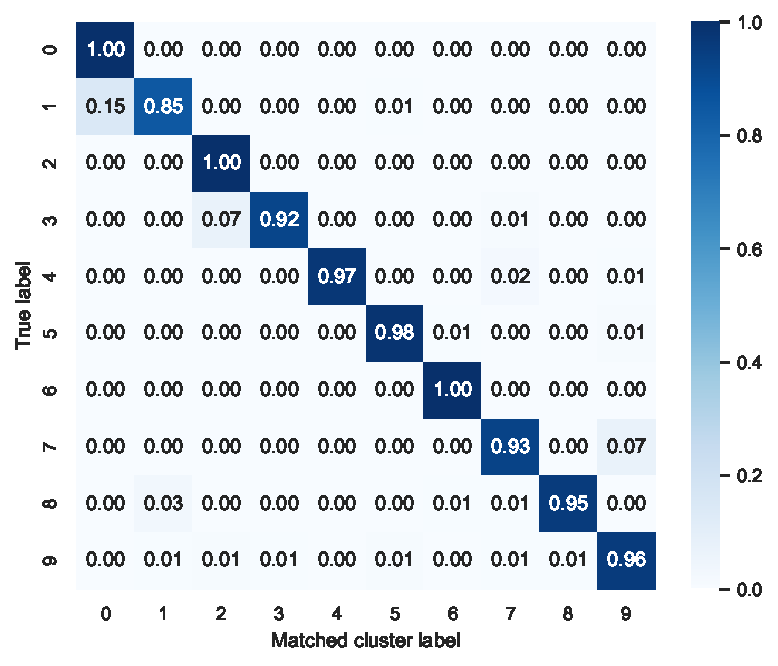
\includegraphics[width=0.48\textwidth]{figures/confusion_proposed.pdf}
    \caption{原始 K-means（左）与本文方法（右）的归一化混淆矩阵}
    \label{fig:confusion}
\end{figure}

本文方法正确聚类 1717 个样本，错误 80 个。主要混淆包括：27 个数字 1 被映射到
数字 0 对应簇，13 个数字 7 被映射到数字 9 对应簇，以及 13 个数字 3 被映射到
数字 2 对应簇。这些样本通常存在闭合笔画、顶部横线或尾部弯曲等相似局部结构。
与基线相比，本文方法的对角线明显集中，但硬聚类仍无法表达少量处于类别过渡区域的
模糊样本。

\section{创新点总结}

本文创新不依赖深度预训练模型，核心改进均可解释并具有对应消融证据：

\begin{enumerate}
    \item 将图像矩倾斜校正引入无监督数字聚类，减少书写姿态造成的类内差异；
    \item 使用样本局部邻域距离定义自适应图权重，适应不同数字的密度变化；
    \item 提出以原始邻域图模块度选择谱空间 K-means++ 重启结果，替代与图目标
    不一致的最小欧氏惯性准则；
    \item 使用有限步邻域一致性细化处理局部边界错误，并通过消融验证其作用；
    \item 建立包含 DBSCAN 噪声覆盖率、参数敏感性和多随机种子稳定性的完整评价协议。
\end{enumerate}

\section{实践总结与心得体会}

本次实践最重要的认识是：较高的算法复杂度不等于更好的聚类结果，评价协议和建模假设
更为关键。最初对每个像素进行方差标准化会放大几乎恒定的背景像素，使 K-means 基线
被明显低估；修正预处理后，原始像素 K-means 已达到约 79\% ACC。

第二个认识是内部优化目标必须与模型结构一致。在谱空间中简单选择惯性最小的
K-means 重启，可能得到欧氏意义更紧凑但图结构更差的划分。改用模块度后，参数和
重启结果都可以在无标签条件下选择，准确率和稳定性同时提高。

第三个认识是对 DBSCAN 必须同时报告覆盖率和全样本准确率。只报告非噪声样本上的
条件准确率会掩盖大量样本被拒绝的问题。完整实验应主动呈现算法局限，而不是只选择
有利指标。

\section{结论与展望}

本文完成了一个可复现的手写数字无监督聚类系统。通过倾斜校正、局部尺度谱图、
模块度重启选择和邻域一致性细化，最终 ACC 达到 95.55\%，明显优于 K-means、
DBSCAN、GMM 和标准谱聚类。消融、敏感性和稳定性实验共同验证了改进方法的有效性。

方法的主要局限是需要构建样本图并进行特征分解，数据规模较大时计算和存储成本会
增加；此外，邻域多数投票可能对极少数真实小簇产生过度平滑。未来可研究近似近邻、
Nystr\"om 谱近似、置信度约束的自适应细化，以及在更大手写数据集上的泛化能力。

\nocite{dalal2005,rousseeuw1987}
\reference

\end{document}
